\documentclass{beamer}
\usepackage[utf8]{inputenc}

\usetheme{Madrid}
\usecolortheme{default}
\usepackage{amsmath,amssymb,amsfonts,amsthm}
\usepackage{txfonts}
\usepackage{tkz-euclide}
\usepackage{listings}
\usepackage{adjustbox}
\usepackage{array}
\usepackage{tabularx}
\usepackage{gvv}
\usepackage{lmodern}
\usepackage{circuitikz}
\usepackage{tikz}
\usepackage{graphicx}
\lstset{
  literate={≠}{{$\neq$}}1 {→}{{$\to$}}1
}

\setbeamertemplate{page number in head/foot}[totalframenumber]

\usepackage{tcolorbox}
\tcbuselibrary{minted,breakable,xparse,skins}



\definecolor{bg}{gray}{0.95}
\DeclareTCBListing{mintedbox}{O{}m!O{}}{%
  breakable=true,
  listing engine=minted,
  listing only,
  minted language=#2,
  minted style=default,
  minted options={%
    linenos,
    gobble=0,
    breaklines=true,
    breakafter=,,
    fontsize=\small,
    numbersep=8pt,
    #1},
  boxsep=0pt,
  left skip=0pt,
  right skip=0pt,
  left=25pt,
  right=0pt,
  top=3pt,
  bottom=3pt,
  arc=5pt,
  leftrule=0pt,
  rightrule=0pt,
  bottomrule=2pt,
  toprule=2pt,
  colback=bg,
  colframe=orange!70,
  enhanced,
  overlay={%
    \begin{tcbclipinterior}
    \fill[orange!20!white] (frame.south west) rectangle ([xshift=20pt]frame.north west);
    \end{tcbclipinterior}},
  #3,
}
\lstset{
    language=C,
    basicstyle=\ttfamily\small,
    keywordstyle=\color{blue},
    stringstyle=\color{orange},
    commentstyle=\color{green!60!black},
    numbers=left,
    numberstyle=\tiny\color{gray},
    breaklines=true,
    showstringspaces=false,
}
%------------------------------------------------------------
%This block of code defines the information to appear in the
%Title page
\title %optional
{1.6.28}
%\subtitle{A short story}

\author % (optional)
{AI25BTECH11013-Gautham}


\begin{document}


\frame{\titlepage}
\begin{frame}{Question}
Show that the points $A(-2\hat{i}+3\hat{j}+5\hat{k}),B(\hat{i}+2\hat{j}+3\hat{k}) and C(7\hat{i}-\hat{k})$are collinear. 
\end{frame}

\begin{frame}{Theoretical Solution}
Let the points are $\vec{A}\myvec{-2\\3\\5}$,$\vec{B}\myvec{1\\2\\3}$ and $\vec{C}\myvec{7\\0\\-1}$.
\end{frame}

\begin{frame}{Theoretical Solution}
\begin{align}
\vec{B} - \vec{A} = \myvec{1\\2\\3} - \myvec{-2\\3\\5}  \\
\vec{B} - \vec{A} = \myvec{1-(-2)\\2-3\\3-5} = \myvec{3\\-1\\-2}  \\
\vec{C} - \vec{A} = \myvec{7\\0\\-1} - \myvec{-2\\3\\5}  \\
\vec{C} - \vec{A} = \myvec{7-(-2)\\0-3\\-1-5} = \myvec{9\\-3\\-6}  \\
\end{align}
\end{frame}

\begin{frame}{Theoretical Solution}
If $\vec{A}$, $\vec{B}$ and $\vec{C}$ are collinear, then the Rank of matrix $(\vec{B} - \vec{A},\vec{C} - \vec{A})$ should be 1.

\begin{align}
(\vec{B} - \vec{A},\vec{C} - \vec{A}) = \myvec{3&9\\-1&-3\\-2&-6}  \\ 
R_3 \rightarrow (\frac{R_1}{3}\times2) + R_3  \\
R_2 \rightarrow \frac{R_1}{3} + R_2  \\
= \myvec{3&9\\0&0\\0&0}  \\
\end{align}
\end{frame}

\begin{frame}{Theoretical Solution}
Since all elements of $R_2$ and $R_3$ are 0, The Rank of matrix $(\vec{B} - \vec{A},\vec{C} - \vec{A})$ is 1.  \\
$\implies$ $\vec{A}$, $\vec{B}$ and $\vec{C}$ are collinear.
\end{frame}


\begin{frame}[fragile]
    \frametitle{main C Code}

    \begin{lstlisting}
#include <stdio.h>

int are_collinear(float A[3], float B[3], float C[3]);

int main() {
    float A[3] = {-2, 3, 5};
    float B[3] = {1, 2, 3};
    float C[3] = {7, 0, -1};

    if (are_collinear(A, B, C)) {
        printf("The points are collinear.\n");
    } else {
        printf("The points are not collinear.\n");
    }

    return 0;
}
    \end{lstlisting}
\end{frame}

\begin{frame}[fragile]
    \frametitle{C Code}

    \begin{lstlisting}
#include <stdio.h>

int are_collinear(float A[3], float B[3], float C[3]) {
    float AB[3], AC[3];

    for (int i = 0; i < 3; i++) {
        AB[i] = B[i] - A[i];
        AC[i] = C[i] - A[i];
    }

    float ratio = 0.0;
    int initialized = 0;
    \end{lstlisting}
\end{frame}

\begin{frame}[fragile]
    \frametitle{C Code}

    \begin{lstlisting}
    for (int i = 0; i < 3; i++) {
        if (AC[i] != 0) {
            float current_ratio = AB[i] / AC[i];
            if (!initialized) {
                ratio = current_ratio;
                initialized = 1;
            } else {
                if (current_ratio != ratio) {
                    return 0; // Not collinear
                }
            }
        } else if (AB[i] != 0) {
            return 0; // AC[i] = 0 but AB[i] ≠ 0 → not proportional
        }
    }

    return 1; // Collinear
}
    \end{lstlisting}
\end{frame}

\begin{frame}[fragile]
    \frametitle{Python Code}
    \begin{lstlisting}
import ctypes
import numpy as np
import matplotlib.pyplot as plt

lib = ctypes.CDLL('./func.so')


lib.are_collinear.argtypes = [ctypes.POINTER(ctypes.c_float),
                              ctypes.POINTER(ctypes.c_float),
                              ctypes.POINTER(ctypes.c_float)]
lib.are_collinear.restype = ctypes.c_int

A = np.array([-2, 3, 5], dtype=np.float32)
B = np.array([1, 2, 3], dtype=np.float32)
C = np.array([7, 0, -1], dtype=np.float32)
    \end{lstlisting}
\end{frame}

\begin{frame}[fragile]
    \frametitle{Python Code}
    \begin{lstlisting}

result = lib.are_collinear(A.ctypes.data_as(ctypes.POINTER(ctypes.c_float)),
                           B.ctypes.data_as(ctypes.POINTER(ctypes.c_float)),
                           C.ctypes.data_as(ctypes.POINTER(ctypes.c_float)))

if result == 1:
    print("Points are collinear")
else:
    print("Points are NOT collinear")

fig = plt.figure()
ax = fig.add_subplot(111, projection='3d')
    \end{lstlisting}
\end{frame}

\begin{frame}[fragile]
    \frametitle{Python Code}
    \begin{lstlisting}
ax.scatter(*A, color='red', label='A')
ax.scatter(*B, color='green', label='B')
ax.scatter(*C, color='blue', label='C')

ax.plot([A[0], B[0]], [A[1], B[1]], [A[2], B[2]], 'gray', linestyle='--')
ax.plot([A[0], C[0]], [A[1], C[1]], [A[2], C[2]], 'gray', linestyle='--')

ax.set_xlabel('X')
ax.set_ylabel('Y')
ax.set_zlabel('Z')
ax.legend()
plt.title("Visualization of Points A, B, and C")
plt.savefig("/home/gauthamp/ee1030-2025/ai25btech11013/matgeo/1.6.28/figs/Fig 1.png")
plt.show()
    \end{lstlisting}
\end{frame}

\begin{frame}{Plot}
    \centering
    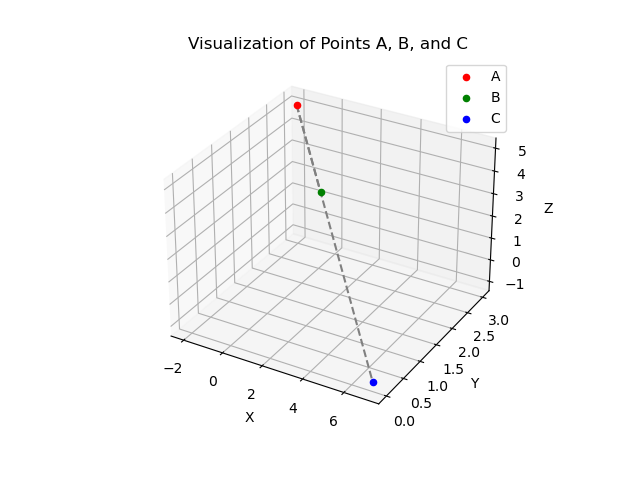
\includegraphics[width=\columnwidth, height=0.8\textheight, keepaspectratio]{figs/Fig 1.png}     
\end{frame}

\end{document}
